\documentclass[landscape,pdftex]{jomislides}

\slidesmag{5} % escala, qto maior maiores ser�o as letras/figras/etc.

%\centerslidesfalse

%\usepackage{algorithmic}
\usepackage{alltt}
\usepackage{booktabs}
%\usepackage{algorithm}

\begin{document}

%\input{autorHeaders}

\title{Web Data Mining com R: design de projetos para cria��o de modelos preditivos} 
\author{Fabr�cio Jailson Barth}
\institution{Faculdade BandTec e VAGAS Tecnologia}
\date{Junho de 2013}

\SlideHeader{}
            {}
\SlideFooter{\theslidepartheading $\;$ --- $\;$ \theslideheading}
            {\theslide}

\vpagecolor[white]{white}


\subtitle{}

\maketitle

\begin{Slide}{Sum�rio e Objetivos}
\begin{itemize}
\item Etapas em estudos preditivos
\item Escolha dos dados
\item Medidas de erro
%\item O problema de \textit{overfitting} e \textit{underfitting}
\end{itemize}
\end{Slide}


\begin{Slide}{Etapas em estudos preditivos}
\begin{itemize}
\item Escolher o conjunto de dados corretos.

%\item Definir a taxa de erro aceit�vel.
\item Dividir os dados em:

\begin{itemize}
\item Treinamento.
\item Teste.
\item Valida��o (opcional).
\end{itemize}

\newpage

\item Selecionar atributos que devem formar o conjunto de treinamento.

\item Identificar modelos preditivos usando o conjunto de treinamento.

\newpage

\item Aplicar \textit{cross-validation} sobre o conjunto de
  treinamento.

\item Se n�o existe conjunto de valida��o ent�o aplicar o modelo 1x no
  conjunto de teste.

\item Se existe conjunto de valida��o ent�o aplicar o modelo no
  conjunto de teste e refinar o modelo.

\item Se existe conjunto de valida��o ent�o aplicar o modelo 1x no
  conjunto de valida��o.

\end{itemize}
\end{Slide}


\begin{Slide}{Identificando o conjunto de dados corretos}
\begin{itemize}
\item Em alguns casos � f�cil (avalia��o de filmes $\rightarrow$ novas
  avalia��es de filmes).
\item Em outros pode ser mais dif�cil (dados gen�ticos $\rightarrow$ doen�as).

\item Geralmente, quanto maior a quantidade de dados, melhor s�o os
  modelos.

\item Conhecer \textit{bench marks} ajuda!

\item \emph{Sempre come�amos com dados brutos e precisamos process�-los}.

\end{itemize}
\end{Slide}

\begin{Slide}{Defini��o de Erro}

\begin{table}[htpb]
\centering
\tiny
\caption{Conjunto de teste}
\vspace{0.2cm}
\begin{tabular}{|l|c|c|}
\toprule
Exemplo & Classe real & Classe inferida\\
\midrule
1 & Positivo & Positivo\\
2 & Positivo & Negativo\\
3 & Negativo & Negativo\\
4 & Negativo & Negativo\\
5 & Negativo & Negativo\\
6 & Positivo & Positivo\\
7 & Positivo & Negativo\\
8 & Negativo & Negativo\\
\bottomrule
\end{tabular}
\end{table}

\newpage

\begin{equation}
erro(modelo) = \frac{qtd\_incorretos}{qtd\_exemplos}
\end{equation}

onde:
\begin{itemize}
\item $qtd\_exemplos$: quantidade de exemplos do conjunto de teste.
\item $qtd\_corretos$: quantidade de exemplos do conjunto de teste
  incorretamente classificados. 
\end{itemize}

\newpage

Neste exemplo:

\begin{table}[htpb]
\centering
\tiny
\caption{Conjunto de teste}
\vspace{0.2cm}
\begin{tabular}{|l|c|c|}
\toprule
Exemplo & Classe real & Classe inferida\\
\midrule
1 & Positivo & Positivo\\
2 & Positivo & Negativo\\
3 & Negativo & Negativo\\
4 & Negativo & Negativo\\
5 & Negativo & Negativo\\
6 & Positivo & Positivo\\
7 & Positivo & Negativo\\
8 & Negativo & Negativo\\
\bottomrule
\end{tabular}
\end{table}

\begin{equation}
erro(modelo) = \frac{2}{8} = 0.25
\end{equation}

\end{Slide}

\begin{Slide}{Defini��o de Verdadeiro e Falso Positivo}
\begin{itemize}
\item Verdadeiro Positivo = identificado corretamente.
\item Falso Positivo = identificado incorretamente.
\item Verdadeiro Negativo = rejeitado corretamente.
\item Falso Negativo = rejeitado incorretamente.
\end{itemize}

\newpage

Exemplo de teste m�dico:

\begin{itemize}
\item Verdadeiro Positivo = Pessoa doente corretamente classificada
  como doente.
\item Falso Positivo = Pessoa saud�vel incorretamente classificada
  como doente.
\item Verdadeiro Negativo = Pessoa saud�vel corretamente classificada
  como saud�vel. 
\item Falso Negativo = Pessoa doente incorretamente classificada como
  saud�vel.  
\end{itemize}

\end{Slide}


\begin{Slide}{Matriz de precis�o e cobertura}

\begin{table}[htpb]
\centering
\tiny
\vspace{0.2cm}
\begin{tabular}{|l|l|l|c|}
\toprule
& \textbf{Positivo de fato} & \textbf{Negativo de fato} & \textbf{Precis�o}\\
\midrule
\textbf{Classificados} & Verdadeiro  & Falso & \\
\textbf{pelo modelo} & Positivo & Positivo & $VP / (VP + FP)$\\ 
\textbf{como positivo} & (VP)  &  (FP) & \\
\midrule
\textbf{Classificados} & Falso & Verdadeiro & \\
\textbf{pelo modelo} & Negativo & Negativo & $VN / (VN + FN)$\\
\textbf{como negativo} & (FN) & (VN) & \\
\midrule
\textbf{Cobertura} & & & Acur�cia: \\
& $VP / (VP + FN)$ & $VN / (FP + VN)$ & $(VP + VN) / (FP + FN)$\\
\bottomrule
\end{tabular}
\end{table}
\end{Slide}

\begin{Slide}{\textit{Cross-validation}}
\begin{figure}[htbp]
\centering 
\resizebox*{0.8\columnwidth}{0.8\textheight}
{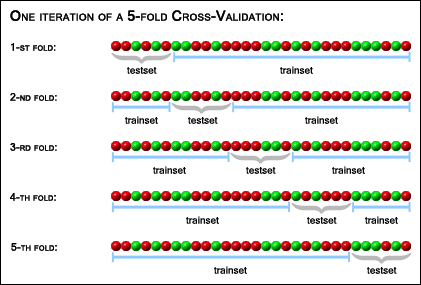
\includegraphics{figuras/crossValidation.png}}
\end{figure}
\end{Slide}

%\begin{Slide}{Os problemas de \textit{overfitting} e \textit{underfitting}}
%\begin{itemize}
%\item 
%\item 
%\end{itemize}
%\end{Slide}

\begin{Slide}{Material de \textbf{consulta}}
  \begin{itemize}
  \item Tom Mitchell. Machine Learning, 1997. (Cap�tulo 5).
  \item Iah H. Witteh and Eibe Frank. Data Mining, 2000. (Cap�tulo 5).
  \item \textit{Prediction study design. Data Analysis
      Course}. Coursera.org
  \item Imagens retiradas de 
   http://genome.tugraz.at/proclassify/help/pages/XV.html 
  \end{itemize}
\end{Slide}


\end{document}

